% =========================================================================== %
% Scout Tooling
% =========================================================================== %

\ifx\wholebook\relax\else
  \documentclass[a4paper,10pt,twoside]{book}
  %=============================================================================%
% Common things, settings, packages to include
%=============================================================================%

\usepackage{graphicx}
\usepackage{color}
\usepackage{makeidx}
\usepackage{ifpdf}
\usepackage{verbatim}

% --------------------------------------------------------------------------- %
% Setting up stuff depeding on output format
% --------------------------------------------------------------------------- %

\ifpdf
  % special settings for pdf mode
  \usepackage[colorlinks]{hyperref}
  \usepackage{courier}
  
  \hypersetup{
    colorlinks,
    linkcolor=darkblue,
    citecolor=darkblue,
    pdftitle={The Eclipse Scout Book},
    pdfauthor={The Scout Community},
    pdfkeywords={Enterprise Framework, Eclipse, Java, Client-Side, Rich Client, Web Client, Mobile},
    pdfsubject={Computer Science}
  }
  
  \usepackage{caption}
  \captionsetup{margin=10pt,font=small,labelfont=bf}
\else
  % special stuff for html mode
  \usepackage[tex4ht]{hyperref}
\fi

% --------------------------------------------------------------------------- %
% Setting up printing range
% --------------------------------------------------------------------------- %

\parindent 1cm
\parskip 0.2cm
\topmargin 0.2cm
\oddsidemargin 1cm
\evensidemargin 0.5cm
\textwidth 15cm
\textheight 21cm

% --------------------------------------------------------------------------- %
% Setting up listings
% --------------------------------------------------------------------------- %

\usepackage{listings}
 
\definecolor{darkviolet}{rgb}{0.5,0,0.4}
\definecolor{darkgreen}{rgb}{0,0.4,0.2} 
\definecolor{darkblue}{rgb}{0.1,0.1,0.9}
\definecolor{darkgrey}{rgb}{0.5,0.5,0.5}
\definecolor{lightblue}{rgb}{0.4,0.4,1}
\definecolor{lightgray}{rgb}{0.97,0.97,0.97}

\renewcommand{\lstlistlistingname}{List of Listings}

% general settings
\lstset{
  basicstyle=\small\ttfamily,
  columns=fullflexible,
  breaklines=true,
  breakindent=10pt,
  prebreak=\mbox{{\color{blue}\tiny$\searrow$}},
  postbreak=\mbox{{\color{blue}\tiny$\rightarrow$}},
  showstringspaces=false,
  backgroundcolor=\color{lightgray}
}

% settings for xml files
\lstdefinelanguage{xml}
{
  commentstyle=\color{darkgrey}\upshape,
  morestring=[b]",
  morestring=[s]{>}{<},
  morecomment=[s]{<?}{?>},
  stringstyle=\color{black},
  identifierstyle=\color{darkblue},
  keywordstyle=\color{cyan},
  morekeywords={xmlns,name,point,factory,class}% list your attributes here
}

% settings for ini files
\lstdefinelanguage{ini}
{
  morecomment=[f][\color{darkgrey}\upshape][0]\#, % # is comment iff it's the first char on the line
  stringstyle=\color{black}
}

% default settings (for java files)
\lstset{
  language=Java,
  emphstyle=\color{red}\bfseries,
  keywordstyle=\color{darkviolet}\bfseries,
  commentstyle=\color{darkgreen},
  morecomment=[s][\color{lightblue}]{/**}{*/},
  stringstyle=\color{darkblue},
}

% --------------------------------------------------------------------------- %
% cross reference macros
% --------------------------------------------------------------------------- %
\newcommand{\applabel}[1]{\label{apx:#1}}
\newcommand{\chalabel}[1]{\label{cha:#1}}
\newcommand{\seclabel}[1]{\label{sec:#1}}
\newcommand{\lstlabel}[1]{\label{lst:#1}}
\newcommand{\figlabel}[1]{\label{fig:#1}}
\newcommand{\tablabel}[1]{\label{tab:#1}}

\newcommand{\appref}[1]{Appendix~\ref{apx:#1}}
\newcommand{\charef}[1]{Chapter~\ref{cha:#1}\xspace}
\newcommand{\secref}[1]{Section~\ref{sec:#1}}
\newcommand{\lstref}[1]{Listing~\ref{lst:#1}\xspace}
\newcommand{\figref}[1]{Figure~\ref{fig:#1}\xspace}
\newcommand{\tabref}[1]{Table~\ref{tab:#1}\xspace}

% --------------------------------------------------------------------------- %
% graphics paths
% --------------------------------------------------------------------------- %
\graphicspath{
  {figures/}
  {Introduction/figures/}
}

%=============================================================================%

  \pagestyle{headings}
  \graphicspath{{figures/} {../figures/}}
  \begin{document}
  \sloppy
\fi

% --------------------------------------------------------------------------- %
\chapter{Scout Tooling}
\chalabel{tooling}

In addition to the Scout runtime framework presented in the previous chapter, Eclipse Scout also includes a comprehensive tooling, the Scout SDK. 
Thanks to this tooling, developing Scout applications is made simpler, more productive and also more robust. 
Initially, a solid understanding of the Java language is sufficient to start developing Scout applications and only a rough understanding of the underlying Eclipse/OSGi/JEE technologies is required. 

The Scout SDK consists of navigation support for the application model defined by the Scout runtime and provides many intuitive component wizards. 
This creates an ideal environment to beginners for building complete, high-quality Scout applications. 
Typically, Java developers only need a few days of Scout training to start creating their own advanced client server business applications. 

The Scout SDK also helps developers to become more productive.
Many repetitive and error prone tasks run automatically in the background or are taken care of by the component wizards of the Scout SDK. 
This starts with the initial creation of a Scout client server application, continues with the wizards to create complete dialogs and pages and includes the automatic management of the data transfer objects needed by the client server communication.

Finally, the application code created by the Scout SDK wizards helps to ensure that the resulting Scout application has a consistent and robust code base and is well aligned with the application model defined by the Scout runtime framework.

% --------------------------------------------------------------------------- %
\section{The Scout SDK}

The Scout SDK is added to the Eclipse IDE in the form of the Scout perspective\footnote{
See \appref{eclipse_perspective} for additional information regarding Eclipse IDE perspectives. 
}.
With the Scout Explorer and Scout Objects Properties, two view parts are contained in the Scout perspective. 
Additionally, the Scout SDK contains a comprehensive set of wizards that support the developer in creating Scout application components. 

The Scout Explorer view allows the developer to navigate the complete Scout application model. 
Once an element in the Scout Explorer is selected, the Scout Object properties view allows to view and change selected properties of the selected element. 
Depending on the selected element in the Scout Explorer, the Scout SDK offers appropriate context menues to start the related wizards.

\begin{figure}
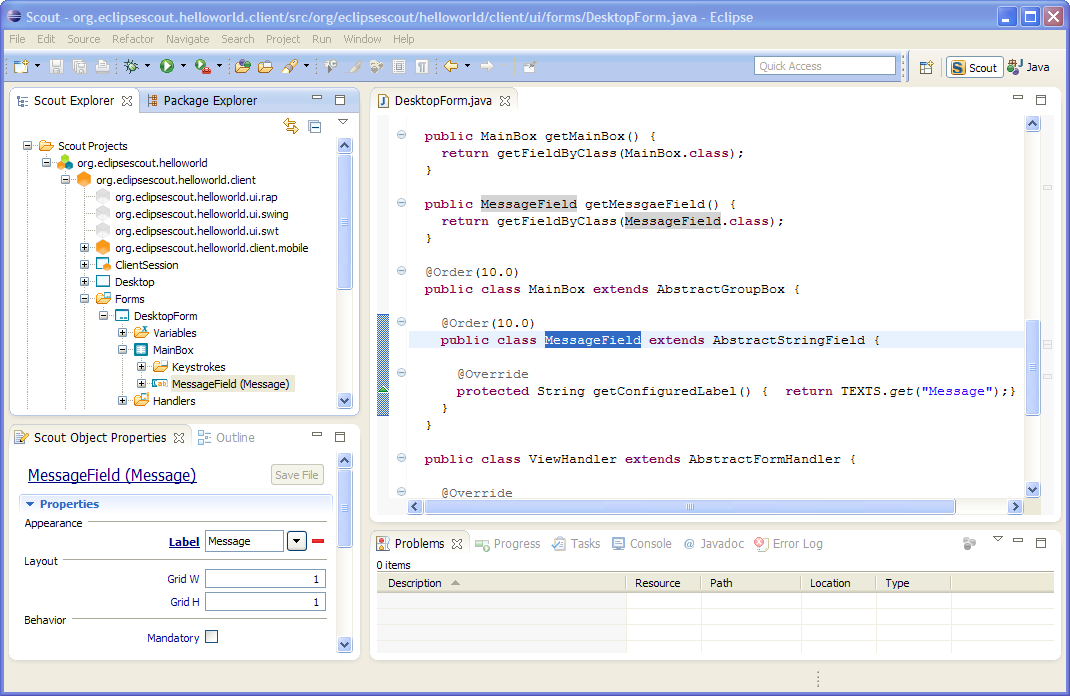
\includegraphics[width=14cm]{scout_sdk_perspective.png} 
\caption{The Scout SDK perspective. On the left hand side the Eclipse Scout Explorer and the Scout Object Properties view are visible.}
\figlabel{scout_sdk_perspective}
\end{figure}

\figref{scout_sdk_perspective} provides a screenshot of the Scout SDK perspective. 
In the Eclipse Scout Explorer shown in the upper left part of the screenshot, the message field in the desktop form of the ''Hello World'' application is selected. 
In the Scout Object Properties located below, the message field's appearance, layout and behaviour properties are displayed. 
On the right side, the corresponding source code is loaded in a Java editor. 

When the developer changes a property of the selected element, the Java code is updated accordingly. 
For example, clicking the \property{Mandatory} in the Scout Object Properties of the message field will insert the method \java{getConfiguredLabel} to the message field's class. 
This demonstrates how the Scout SDK directly works on the Java source code. 
In fact, the Java source code is the only artefact relevant for the Scout SDK to 'understand' the Scout application model. 
Taking advantage of this setup, the Scout SDK implements a full round-trip-engineering from creating the Java code for Scout application components, parsing code changes in the background, and displaying the current implementation of the Scout application in the Scout Explorer and the Scout Object Properties.

Thanks to the round-trip-engineering provided by the Scout SDK, the information presented in the Scout Explorer and the Scout Object Properties always stay in sync with the Java code of the Scout application.
To illustrate this, we will re-use the ''Hello World'' Scout project from \charef{helloworld}. 
Start the Eclipse IDE with the workspace containing the ''Hello World'' application.
Then, navigate to method \java{getConfiguredLabel} as shown in \figref{scout_sdk_perspective}, and add the java snippet shown below to the class \java{MessageField}. 

\begin{lstlisting}[backgroundcolor=\color{white}]
    @Override
    protected boolean getConfiguredMandatory() {
        return true;
    }
\end{lstlisting}

After having saved the code change, you can observe that the \property{Mandatory} in the section Behaviour of the message field's Scout Object properties has changed its state. 
The font of its label is now presented in bold face and underlined, the checkbox is ticked and a red minus icon is shown on the right side of the property. 
Obviously, the Scout SDK is directly operating on the project's source code and does not rely or need any external meta data. 
This provides the flexibility to develop Scout applications with or without the support of the Scout SDK. 
And this choice offered to the Scout developer is one of the most important features provided by the Scout SDK. 
The Scout developer may take advantage of the development support provided by the Scout SDK without being restricted by the Scout tooling in any way.

Technically, the Scout SDK is a set of Eclipse plugins that operate on top of the Eclipse JDT and the Eclipse PDE projects.
The Java Development Tools (JDT)\footnote{
See the Eclipse JDT project page for details: \url{http://www.eclipse.org/jdt/}.
} 
contain a Java IDE supporting the development of any Java application, 
and the Plugin Development Environment (PDE)\footnote{
See the Eclipse PDE project page for details: \url{http://www.eclipse.org/pde/}.
}
provides tools to create, develop, test, debug, build and deploy Eclipse plugins, and additional artefacts relevant for Eclipse based applications. 
As in the case of the Scout Runtime, the plugins representing the Scout SDK, the JDT and the PDE are all located in the \filename{plugins} directory your Eclipse installation and named \filename{org.eclipse.scout.sdk.*}, \filename{org.eclipse.jdt.*} and \filename{org.eclipse.pde.*} . 

% --------------------------------------------------------------------------- %
\section{The Scout Explorer}

The Scout Explorer view is responsible for the navigation support within the Scout application model. 
This navigation support is presented in the form of a tree view and includes the client with its UI components, the server and the shared part of a Scout application. 
It also includes all Scout application modules of modular Scout applications\footnote{
See \secref{multi_module_apps} for more information regarding multi module Scout applications.
}.
For the actual navigation in the tree representing the Scout application both the mouse or the keyborad can be used. 

To expand or collapse a selected node in the Scout Explorer, you may click on the tiny \icon{plus} or the \icon{minus} presented to the left of the node.
Alternatively, you can also use the \key{Right} or the \key{Left}.

Once a node in the tree is selected, the Scout Object Properties view presents the associated configuration of the selected element. 
If the selected element represents a specific application model component, the corresponding Java source code can be accessed through a double click on the node, or hitting the \key{Enter}. 

The navigation tree provided in the Scout Explorer view also allows the developer to add elements to your application.
Depending on the selected node in the tree, the Scout SDK allows to start the applicable Scout SDK wizards using corresponding context menus. 
The wizards support the creation of application components, such as dialogues on the client side or services on the server side by generating the necessary Java code.

\begin{figure}
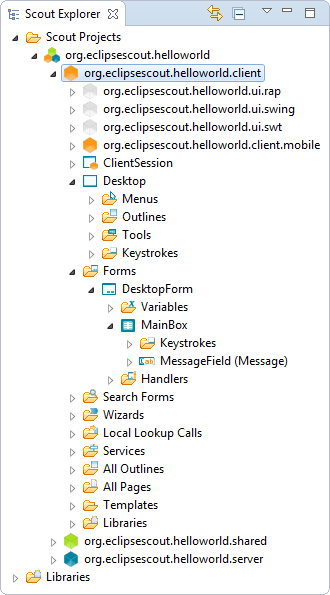
\includegraphics[width=6.5cm]{explorer_client.png} 
\caption{The Scout Explorer view. The white nodes below the expanded client node represent the supported UI technologies.}
\figlabel{explorer_client}
\end{figure}

In \figref{explorer_client} the top level organisation of the client application model is shown as it is represented in the Scout Explorer.
All client specific elements are located under the selected orange client node \element{org.eclipsescout.helloworld.client}. 
Right below, the three white UI plugins are located that represent the support for the corresponding UI technolgies for Swing, SWT and Eclipse RAP. 
The orange \node{org.eclipsescout.helloworld.client.mobile} contains all elements that are specific to mobile devices such as the \java{MobileHomeForm}

Specific nodes for the client session and the desktop of the Scout client allow access to the corresponding Scout application model components. 
While the client session is the main entry point for client-server communication, the desktop represents the root component of the visible part of a Scout client applications. 
Below, a set of folders group additional client model components according to their type. 
The forms folder for example holds all available forms, such as the desktop form that we have seen in the ''Hello World!'' tutorial\footnote{
See \secref{initial_helloworld} for a description of many of these elements.
}. 

\begin{figure}
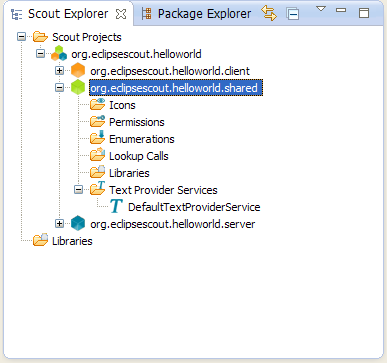
\includegraphics[width=7cm]{explorer_shared.png} 
\caption{The Scout Explorer view with the expanded shared node.}
\figlabel{explorer_shared}
\end{figure}

A screenshot of the expanded green shared node \element{org.eclipsescout.helloworld.} is provided in \figref{explorer_shared}. 
As the name ''shared'' suggests, the corresponding plugin holds all application components that are required for both the Scout client and the Scout server application. 
This includes texts, icons, enumeration or codes, permissions, lookup calls. 
As shown in \figref{explorer_shared}, a separate folder for each resource type is provided under the shared node.
 
\begin{figure}
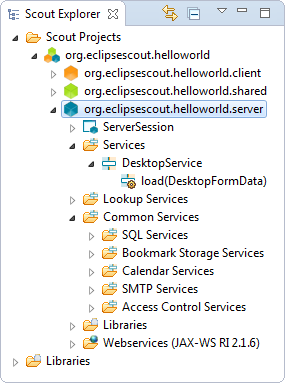
\includegraphics[height=6.8cm]{explorer_server.png} \hspace{5mm} 
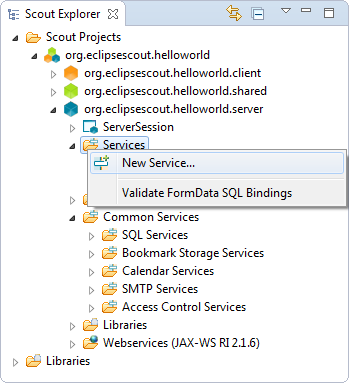
\includegraphics[height=6.8cm]{explorer_server_servicewizard.png}
\caption{The Scout Explorer view with the expanded server node (left). On the individual nodes, access to the relevant Scout SDK wizards is provided via context menues (right).}
\figlabel{explorer_server}
\end{figure}

In \figref{explorer_server}, the blue server node is expanded in the Scout Explorer view. 
As the primary responsibility of the Scout server application is dealing with requests, its components are mostly related to different types of services. 
Below the server session node, the \folder{Services} holds services related to the processing logic of the application such as retrieving and updating data. 
The remaining folder group differnt more specific types of server services. 
Under the \folder{Webservices} the Scout SDK support to provide and consume web services is located. 

The right side of \figref{explorer_server} illustrates the access to the Scout SDK wizards via corresponding context menus. 
The \menu{New Service...} shown in the screenshot will start the wizard to add a new Scout server service. 
 
The different colored tree nodes discussed above are all represented by their individual Eclipse plugins. 
This includes the orange client node, the white UI nodes, the orange mobile client node, the green shared node and the blue server node. 
A Scout Swing client for example contains the plugins \element{org.eclipsescout.helloworld.client}, \element{org.eclipsescout.helloworld.shared} and \element{org.eclipsescout.helloworld.client.ui.swing} but not the other UI technology plugins. 
The Scout server contains the \element{org.eclipsescout.helloworld.server} plugin and the \element{org.eclipsescout.helloworld.shared} plugin. 

% --------------------------------------------------------------------------- %
\section{The Scout Object Properties}

The Scout Object Properties view provides direct access to configurable properties and operations for the element selected in the Scout Explorer.
Before we discuss the typical layout of an object property view we describe the special case of the property view for a complete Scout application. 
This property view is displayed when the application's top level node is selected in the Scout Explorer as shown in \figref{sdk_initial_helloworld_project}. 

\begin{figure}
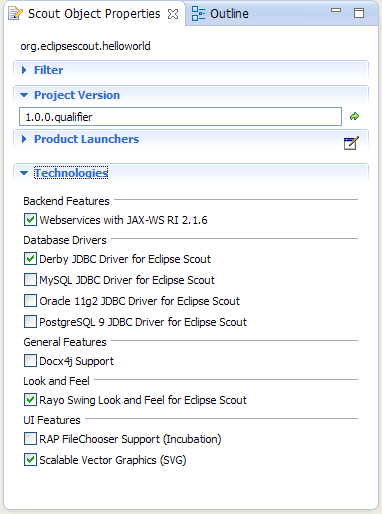
\includegraphics[width=7cm]{properties_technologies.png}
\caption{The Scout Object Properties showing the expanded Technologies section.}
\figlabel{properties_technologies}
\end{figure}

The main elements of the top-level application proprties are the sections \element{Product Launchers} and the \element{Technologies}. 
As the product launcher section with its launcher boxes has alredy been covered in \secref{run_initial} and \secref{run_initial_background} we focus on the technologies section here.
The technologies section allows to add Scout runtime features and functionalities to the Scout application or remove such elements from the application. 

When the selection of a technology checkbox is changed, a message box is shown to the user. 
This box lists all project resources that are changed when the user confirms the action. 
Once the dialog is confirmed, the selected resources are modified by the Scout SDK to add or remove the feature. 

For features containing licences not compatible to the Eclipse Public Licence (EPL) or features in incubation status, the necessary artefacts is not provided as part of the Eclipse Scout installation package. 
Instead, the associated artefacts need to be installed from a remote updated site first. 
Before any non-EPL content is downloaded from the internet, the user needs to review and confirm the associated licence. 
For this, a license confirmation dialog is shown upfront. 
After confirmation, the required files are downloaded and automatically installed in the local Eclipse instance of the developer. 
Usually, the Eclipse IDE needs to restart after a feature is downloaded and installed for the first time. 
Currently, the procedure described above is used for the following technolgies. 

\begin{itemize}
  \item MySQL JDBC Driver for Eclipse Scout
  \item Oracle 11g2 JDBC Driver for Eclipse Scout
  \item PostgresSQL 9 JDBC Driver for Eclipse Scout
  \item Docx4j Support
  \item Rayo Swing Look and Feel for Eclipse Scout
  \item RAP FileChooser Support (Incubation)
\end{itemize}

\begin{figure}
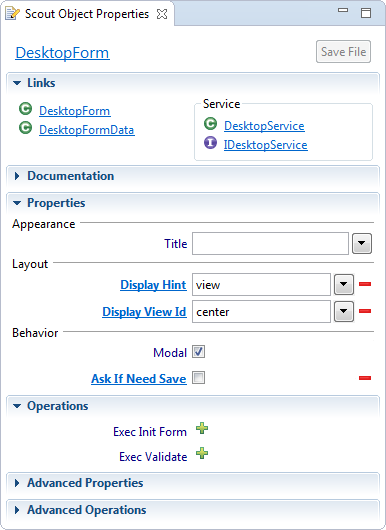
\includegraphics[width=7cm]{properties_form.png} \hspace{5mm}
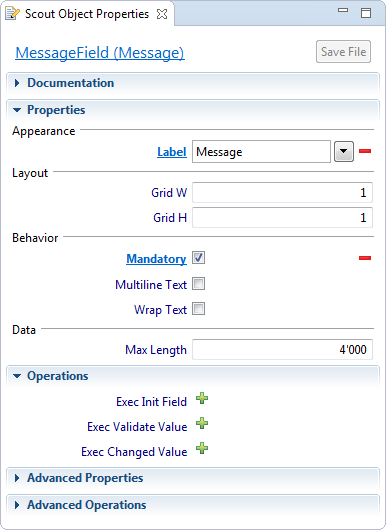
\includegraphics[width=7cm]{properties_stringfield.png}
\caption{The Scout Object Properties for a complete form (left) and a string form field (right).}
\figlabel{properties_view_examples}
\end{figure}

For the description of the Scout Object Properties of typical Scout components we use the example views provided in \figref{properties_view_examples}. 
Both Scout Object Properties example views for the desktop form and the message field are take from the ''Hello World!'' application described in \charef{helloworld}. 
As in the case of the top-level node representing the complete Scout application, the typical layout of the Scout Object Properties view is organized into several sections. 
The content and ordering of the property sections always follows the same scheme.

\begin{itemize}
  \item Filter
  \item Links
  \item Properties
  \item Operations
  \item Advanced Properties
  \item Advanced Operations
\end{itemize}

If a folder node (such as the \folder{Forms} under the orange client node), is selected in the Scout Explorer, the Scout Object Properties only shows a filter section with a filter field. 
The content in this filter field then restricts the elements below the folder icon accordingly. 
This feature is especially useful for the development of larger applications containing dozens of forms or services. 

The \element{Links} section provides a set of hyperlinks as shown on the left hand side of \figref{properties_view_examples}. 
The provided links all refer to Java classes and interfaces that related to the Scout component represented by the property view. 

The available properties of a Scout component are listed in sections \element{Properties} and \element{Advanced Properties}. 
Basically, all available Java \java{getConfigured} methods of a Scout component are listed in one of the two sections depending on the frequency of their usage. 
Section \element{Properties} shows the often used properties, while the less frequently used properties are provided in section \element{Advanced Properties}. 
The examples in \figref{properties_view_examples} show the thematical organization of the sections into \element{Appearance}, \element{Layout}, \element{Behaviour} and other groups.

Access to object operations implemented with Java \java{exec} methods is provided in sections \element{Operations} and \element{Advanced Operations}. 
Again, the more and less frequently used operations are assigned to individual sections. 

For all listed properties and operations the corresponding Javadoc is displayed in the form of a tooltip window. 
To display the available Javadoc, move the mouse pointer over the method of interest in the Scout Object Properties\footnote{
This features is work in progress, as for some methods shown in the Scout Object Properties the Javadoc content is not yet available. 
}. 

% organisation of properties and operations defined in file \filename{sdkPropertyViewConfig.xml} 
% of plugin \filename{org.eclipse.scout.sdk.ui_3.9.0.20130529-1904.jar}
% might be worth a footnote or similar?

So far, we did only describe the content and organisation of the Scout Object Properties. 
In the reminder of this section we will describe the procedure to change or update the default values of properties or the default behaviour of Scout components. 
To indicate non-default property values or non-default behaviour, the font of the property or the operation is switched to underlined bold face. 
As an example, consider the property \element{Ask If Need Save} of the desktop form shown on the left side of \figref{properties_view_examples}. 
The bold font visualizes that this does not correspond to the default behaviour of forms. 
And underlining of this property further indicates, that the label has become a clickable link. 
Clicking on this label will load the corresponding method into the Java editor in the Scout SDK. 

To change a property for a specific Scout component just enter a value in the corresponding field or tick/untick the provided checkbox. 
In some cases the value may also be chosen from a dropdown list. 
For the label field shown on the right hand side of \figref{properties_view_examples}, the ''Message'' value refers to the text key to be used in method \java{getConfiguredLabel}. 
To enter a new label text, start typing the desired translated label and pick the option ''New translated text...''. 

To reset a property or operation to its default value/behaviour, you may click on the red \icon{Minus} provided on the right side of the property field. 
This will remove the overridden method from the object's Java code. 

% --------------------------------------------------------------------------- %
\section{Scout SDK Wizards}

The Scout SDK wizards allow the developer to create Scout application model components with just a few clicks. 
Creation wizards are provided for all major model components such as forms on the client side and services on the server side. 
The usage of wizards not only makes developing Scout applications efficient but also helps to create robust code and reduces the number of errors. 

Scout SDK wizards can do many things. 
They add and update Java classes, register services in the \filename{plugin.xml} files, manage plugin dependencies in the \filename{MANIFEST.MF} files and update Eclipse product files when necessary. 
All these capabilities hide a lot of the complexity of writing Eclipse based applications. 
This simplifies the developing of Scout application considerably.

In the text below, descriptions of the most commonly used Scout SDK wizards are provided. 
First, the wizards to create and export complete Scout applications are described. 
Then, the wizards to create Scout application model components are introduced. 

% --------------------------------------------------------------------------- %
\subsection{Creating a new Scout Project}

The \wizard{New Scout Project} allows to create a new Scout client server application. 
In the Scout Explorer, the \contextmenu{New Scout Project...} is provided on the top-level \folder{Scout Projects}. 
The creation of a form based Scout application has already been introduced in \secref{create_project_simple} for the ''Hello World'' tutorial.
And \secref{create_project_simple_background} provides background information related to the artefacts created by this wizard. 
In the text below, we will described the different steps of the creation wizard individually.

\begin{figure}
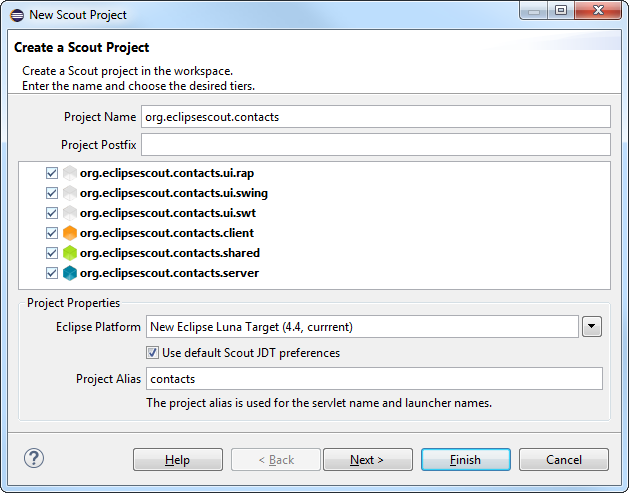
\includegraphics[width=7cm]{wizard_new_project_1.png} \hspace{5mm}
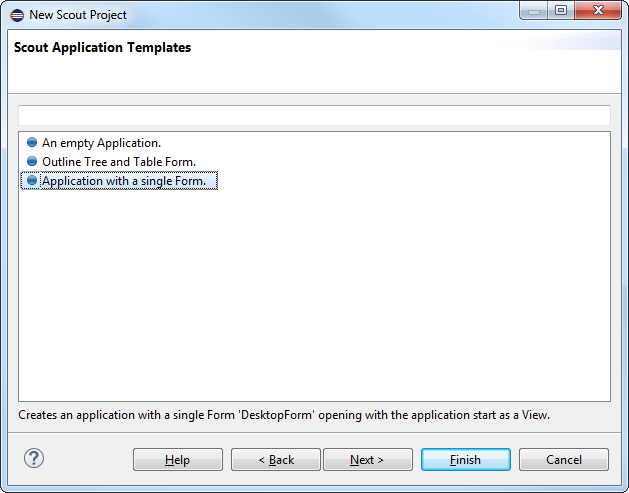
\includegraphics[width=7cm]{wizard_new_project_2.png}
\caption{The Scout wizard to create a new Scout application.
The first wizard dialog (left) is used to specify the needed application plugins. 
In the next wizard step (right) the application template is selected.}
\figlabel{wizard_new_project}
\end{figure}

In the first wizard step shown on the left side of \figref{wizard_new_project}, it is possible to choose:
    The project name: Base name of the project and the plugins that belong to the project.
    The project postfix: An optional postfix to add to the plugin names.
    The project alias: The short name to use for the application. The client executables and server servlet names will use this shortname.
    The JDT preferences: If checked the Scout default Java development settings are copied. Otherwise you start with no settings and can apply your own template. 

The plug-ins (UI Plug-Ins, Client, Shared, Server) are named using the pattern:
 <project name>.<plug in>.<project postfix>

In the checkbox list you can choose which plugin-ins need to be created. A Scout application must not always be a client/server application.
You can also create client only or server only applications. But in any case you must include the shared plug-in in the project.
Because of the separation of the UI and GUI it is possible to choose the UI Plug-ins that will render the application. 

The second wizard step shown on the right side of \figref{wizard_new_project} allows to choose the type of application that should be created. 
Empty Application, This type of application correspond to the minimal application. No additional code is generated. 

Single Form Application, see helloworld tutorial, In this type of application, the main window displays a form. In this example (Swing, Nimbus look and feel, Windows), the menu bar is displayed in this main window on top of the main form.
The SDK creates a form, called DesktopForm. This form comes with a process service (DesktopProcessService) and a form handler (DisplayFormHandler).
With this type of application, there is no default support for outlines and pages. 

Outline based application. Outline based application is the most complete type of application. It is suitable if you want to represent outlines and their pages in the main window. 
In this example (Swing, Nimbus look and feel, Windows) the main window provides: the menu bar, a way to switch between the Outlines attached to the desktop, and a representation of the active outline: on the left hand side the page tree and on the right the selected page. 

\begin{figure}
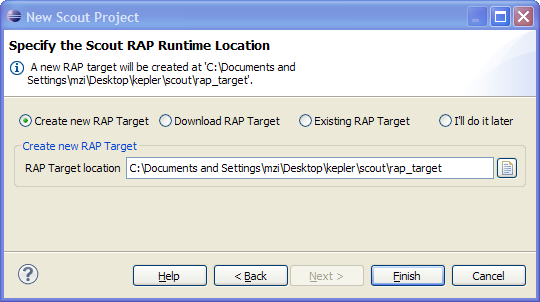
\includegraphics[width=9cm]{wizard_new_project_3.png}
\caption{The last wizard step is used to specify the RAP target for the new Scout application.}
\figlabel{wizard_new_project_rap_target}
\end{figure}

The third wizard step shown in \figref{wizard_new_project_rap_target} is only available if the RAP UI has been checked in Step 1.
Because the RAP runtime cannot be installed into the running Eclipse instance, a separate target platform must be created. 
This target platform must contain all plugins to run the Scout RAP UI. 
There are several possibilities to create such a target platform:

    Create new RAP Target
    This option is only available on an Eclipse with the Scout RAP Target Feature installed in the running Eclipse instance.
    When choosing this option a new RAP target platform will be created at the location specified. This target platform is then defined by all plugins available to the running Eclipse and the RAP target platform extracted to the given directory.
    Download RAP Target
    When choosing this option the target platform will be downloaded into the running workspace. This download will then only be available to the active workspace! There are two download types:
        Only download the RAP plugins (checkbox not ticked, default)
        The target platform will be defined by the plugins available to the running Eclipse instance and the downloaded RAP plugins. This download is smaller.
        Download a new Kepler Eclipse platform as well (checkox ticked)
        A complete, new Kepler target platform will be downloaded and used. This option can be used when you want to ensure that no plugins of the running Eclipse should be in the target platform or if you are not running Eclipse Kepler but want to use Kepler features in your project.
        Be aware that the developer tools in your runnig Eclipse must be compatible with the Kepler platform that will be used then! 
    Existing RAP Target
    An existing RAP target location can be specified. The wizard then tries to detect whether the given location contains a complete target platform or only the RAP target plugins. If a complete platform is detected, only the directory specified will be part of the target platform. Otherwise the given directory together with the plugins available to the running Eclipse will define the target platform.
    I'll do it later
    When choosing this option the Scout SDK does not create a RAP target platform for you. The platform must be created manually after the Scout project has been created. The created project will not compile before a complete target platform has been created! 
	
\noindent Existing Documentation
\begin{itemize}
  \item how-to wiki \url{http://wiki.eclipse.org/Scout/HowTo/3.8/Create_a_new_project}
\end{itemize}

What is a Scout Project?
needs text

\noindent Existing Documentation
\begin{itemize}
  \item forum \url{http://www.eclipse.org/forums/index.php/t/395379/}
  \item wiki concept \url{http://wiki.eclipse.org/Scout/Concepts#Scout_Project}
\end{itemize}

% --------------------------------------------------------------------------- %
\subsection{Exporting a Scout Project}

The \wizard{Export a Scout Project} allows to export a complete Scout client server application as WAR files. 
In the Scout Explorer, the \contextmenu{Export Scout Project...} is provided on the main application node just below the top-level \folder{Scout Projects}. 

\noindent Existing Documentation
\begin{itemize}
  \item forum: access to logs \url{http://www.eclipse.org/forums/index.php/t/367447/}
\end{itemize}

% --------------------------------------------------------------------------- %
\subsection{Creating a Form}

The \wizard{New Form} allows to create a new form including the necessary form data, permissions and server services. 
In the Scout Explorer, the \contextmenu{New Form...} is provided on the \folder{Forms} under the orange client node. 

New Form Field Wizard

% --------------------------------------------------------------------------- %
\subsection{Creating a Form Field}

The \wizard{New Form Field} allows to create a new Scout client server application. 
In the Scout Explorer, the \contextmenu{New Form Field...} is provided on the \node{MainBox} under every form node or nodes representing form field containers, such as group boxes. 

New Form Field Wizard

% --------------------------------------------------------------------------- %
\subsection{Creating a Search Form}

The \wizard{New Search Form} allows to create a new Scout form to search for elements displayed in pages.  
In the Scout Explorer, the \contextmenu{Create Search Form...} is provided on the \folder{Search Forms} under the orange client node. 

New Form Field Wizard

% --------------------------------------------------------------------------- %
\subsection{Creating an Outline}

The \wizard{New Outline} allows to create a new Scout form to search for elements displayed in pages.  
In the Scout Explorer, the \contextmenu{New Outline...} is provided on the \folder{All Outlines} under the orange client node. 
Alternatively, the context menu is also available on the \folder{Outlines} of the \node{Desktop} under the applications client node. 

New Form Field Wizard

% --------------------------------------------------------------------------- %
\subsection{Creating a Page}
needs text

New Form Field Wizard

% --------------------------------------------------------------------------- %
\subsection{Creating a Server Service and Service Operations}

The \wizard{New Service} allows to create a new Scout form to search for elements displayed in pages.  
In the Scout Explorer, the \contextmenu{New Service...} is provided on the \folder{Services} under the orange client node and the blue server node. 
This reflects the fact that services may be defined on both the client and the server side. 

New code type and new code wizards

% --------------------------------------------------------------------------- %
\subsection{Creating Code Types and Codes}
needs text

New code type and new code wizards

% --------------------------------------------------------------------------- %
\subsection{Creating a Permission}
needs text

New permission wizard

% --------------------------------------------------------------------------- %
\subsection{Creating a Library Bundle}
needs text

New library bundle wizard


\ifx\wholebook\relax\else
   \begin{thebibliography}{99}
  \addcontentsline{toc}{chapter}{Bibliography}
  
  % add/insert books in alphabetical order of 1st author
  
  \bibitem{batessierra05}
    \textit{Bert Bates, Kathy Sierra},
	\textbf{Head First Java} 2nd edition, 
	O'Reilly Media, 2005.

  \bibitem{bloch08} 
    \textit{Joshua Bloch},
    \textbf{Effective Java} 2nd edition, 
	Addison-Wesley, 2008.
	
  \bibitem{eckel06}
    \textit{Bruce Eckel},
	\textbf{Thinking in Java} 4th edition, 
	Prentice Hall International, 2006.

\end{thebibliography}

   \end{document}
\fi

% =========================================================================== %
